\chapter{Dialogmodell}

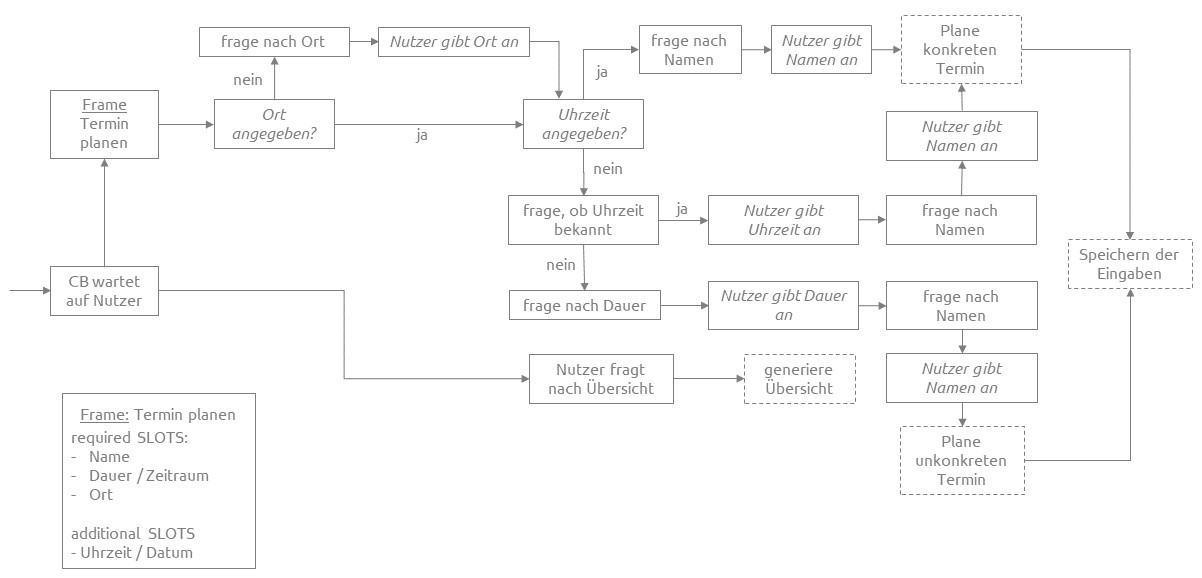
\includegraphics[width=\linewidth]{Dialogmodell_bild}\\
Der Nutzer kann einen Termin planen oder sich seinen derzeitigen Terminplan an Bild anzeigen lassen. Beim Planen von Terminen wird gefragt wo das Event stattfindet, welchen Namen das Event haben soll, ob es ein spezifisches (mit Start- und Endzeit) Event ist oder ein unspezifisches (nur Event-Dauer ist bekannt) und dann der Zeitrahmen/die Dauer.\\
Man kann auch bereits geplante Events wieder löschen. Dabei wählt der Nutzer mit Button, das er löschen will. 
Ein paar Small-Talk Optionen sind auch dabei, wie z.b fragen wie es dem Chatbot geht.\\\\
Der Bot ist eine Mischung aus Frame-basiert und Zustands-basiert. Das Planen von Event ist Frame-basiert, wo nach und nach die Fehlenden Slots (Ort, Event Name, spezifisches/unspezifisches Event,Dauer/Zeitrahmen) gefüllt werden. 
Während des Planens oder des Löschens eines Termins ist der Dialog eher System-Initiated, da die fehlenden Slots abgefragt werden, ansonsten User-Initiated.\\

\newpage
Beispiele:\\ 

\textbf{Plane ein Event mit bestimmtem Zeitrahmen}\\

\begin{framed}
\begin{tabular}{lr}
	\makecell[c]{JANUS} & \makecell[c]{USER} \\
 & plan an event at Rudower Chaussee 25 \\
Okay, what is the name of that event? & \\
 & Uni-Treffen\\
Do you know the exact time? & \\
 & Yes\\
Please tell me the time and date. & \\
 & Tomorrow from 4pm to 5pm\\
 \makecell[l]{Okay. Planned the event Uni-Treffen \\ at Rudower Chaussee 25, 12489 Berlin \\ from 14.08.2919 16:00 - 17:00.}
 \end{tabular}
\end{framed}

\hfill\\
\newpage
\textbf{Plane ein Event mit einer Event-Dauer}\\
\begin{framed}
\begin{tabular}{lr}
	\makecell[c]{JANUS} & \makecell[c]{USER} \\
	& schedule an event\\
	Where will this event take place? &\\
	& at Alten Försterei\\
	Okay, what is the name of that event? & \\
	& Fußball\\
	Do you know the exact time? & \\
	& nope\\
	Please tell me the duration of the event. & \\
	& 2 hours\\
	\makecell[l]{Okay. Planned the event Fußball \\ at Alte Försterei, 12555 Berlin \\ which will take 120min.}
\end{tabular}
\end{framed}
\hfill\\\\\\

\textbf{Erstellten Plan anzeigen lassen}\\
\begin{framed}
	\begin{tabular}{lr}
		\makecell[c]{JANUS} & \makecell[c]{USER} \\
		& please show me what has been scheduled.  \\
		That's what has been scheduled & \\
			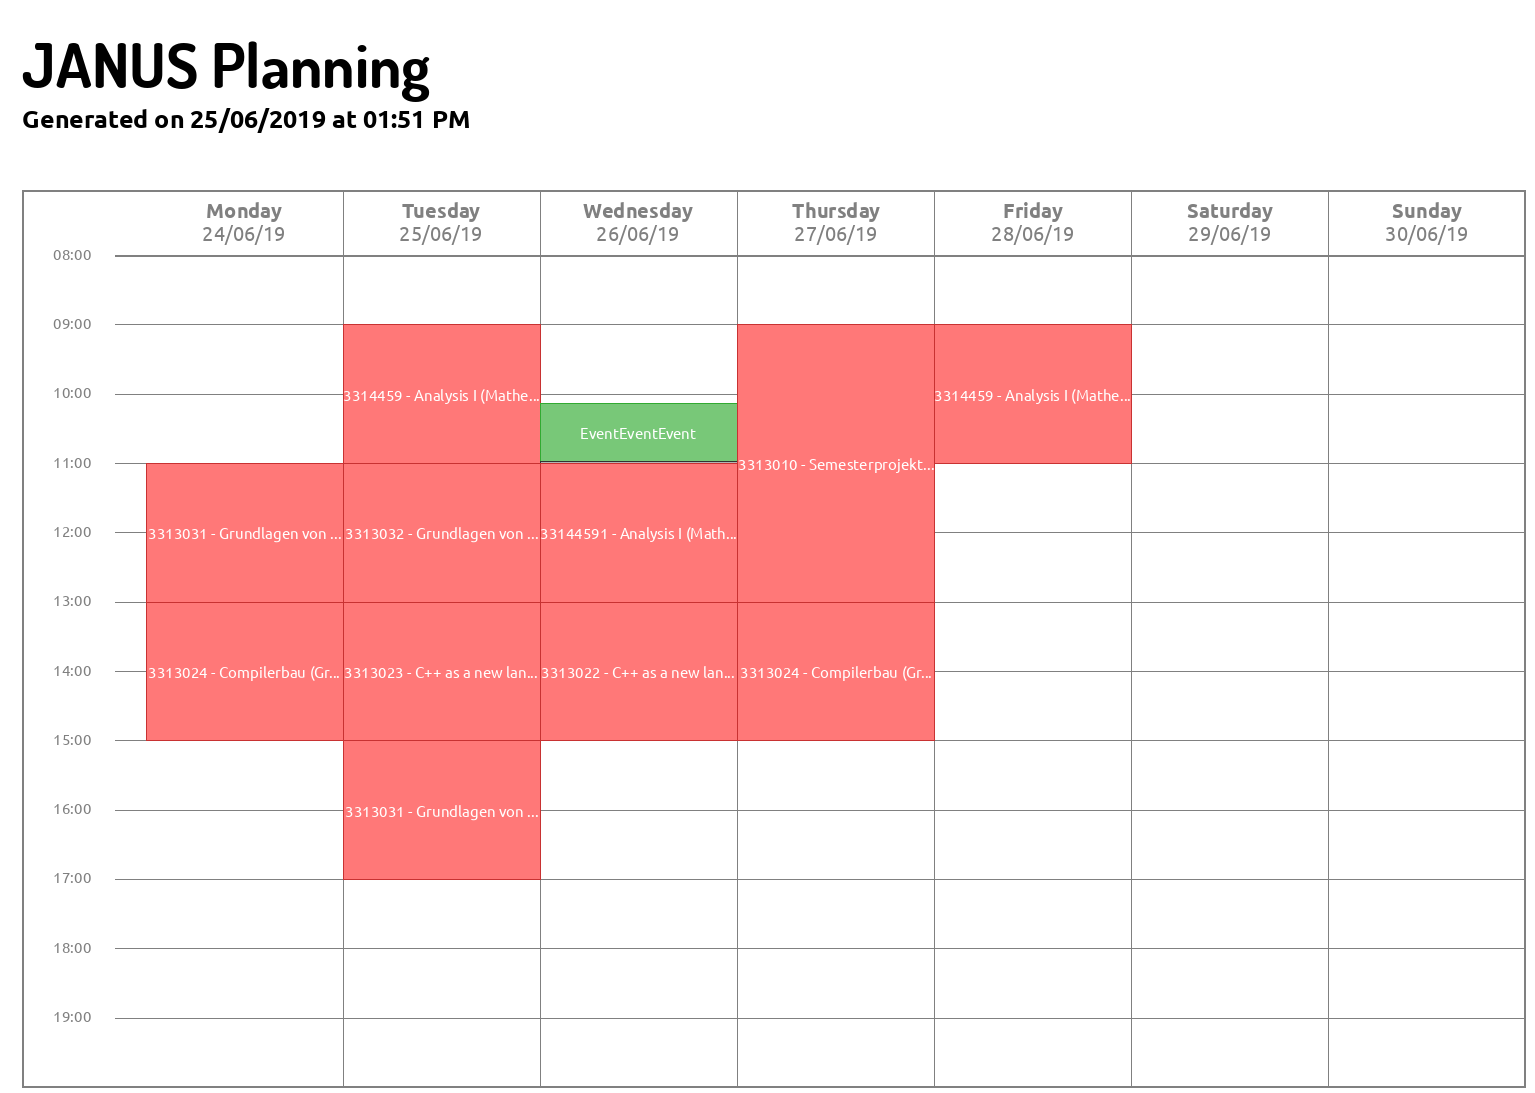
\includegraphics[width=0.30\linewidth]{show_plan} & 
	\end{tabular}
\end{framed}

\begin{framed}
	\begin{tabular}{lr}
		\makecell[c]{JANUS} & \makecell[c]{USER} \\
		& delete an event\\
		Which Event do you want to delete? &\\
			$\qquad$Uni-Treffen  & \\
			$\qquad$Fußball & \\
		& [wählt Fußball aus] \\
		Okay, deleted the event Fußball. & \\
	\end{tabular}
\end{framed}
\hfill\\